% !TEX TS-program = XeLaTeX
% use the following command: 
% all document files must be coded in UTF-8
\documentclass{textolivre}
% See more information on the repository: https://github.com/leolca/textolivre

% Metadata
\begin{filecontents*}[overwrite]{article.xmpdata}
    \Title{Atividades experimentais em tempos de pandemia: o uso da plataforma online PCIBEX para experimentos psicolinguísticos}
    \Author{Aline Alves Fonseca \sep Júlia Greco Carvalho \sep Samara Cristina da Silva Zanella}
    \Language{pt-BR}
    \Keywords{Pesquisa \textit{online} \sep PCIbex \sep Psicolinguística \sep Processamento de sentenças}
    \Journaltitle{Texto Livre}
    \Journalnumber{1983-3652}
    \Volume{14}
    \Issue{3}
    \Firstpage{1}
    \Lastpage{20}
    \Doi{10.35699/1983-3652.2021.27047}

    \setRGBcolorprofile{sRGB_IEC61966-2-1_black_scaled.icc}
            {sRGB_IEC61966-2-1_black_scaled}
            {sRGB IEC61966 v2.1 with black scaling}
            {http://www.color.org}
\end{filecontents*}

\journalname{Texto Livre}
\thevolume{14}
\thenumber{3}
\theyear{2021}
\receiveddate{\DTMdisplaydate{2021}{1}{11}{-1}} % YYYY MM DD
\accepteddate{\DTMdisplaydate{2021}{6}{28}{-1}}
\publisheddate{\DTMdisplaydate{2021}{8}{19}{-1}}
% Corresponding author
\corrauthor{Júlia Greco Carvalho}
% DOI
\articledoi{10.35699/1983-3652.2021.27047}
%\articleid{NNNN} % if the article ID is not the last 5 numbers of its DOI, provide it using \articleid{} commmand
% Abbreviated author list for the running footer
\runningauthor{Fonseca et al.}
\sectioneditorname{Bárbara Amaral da Silva}
\layouteditorname{Anna Izabella M. Pereira}

\title{Atividades experimentais em tempos de pandemia: o uso da plataforma \textit{online} PCIBEX para experimentos psicolinguísticos}
\othertitle{Research activities in the pandemic: the use of the PCIBEX online platform to do psycholinguistics experiments}
% if there is a third language title, add here:
%\othertitle{Artikelvorlage zur Einreichung beim Texto Livre Journal}

\author[1]{Aline Alves Fonseca \orcid{0000-0002-7874-2878} \thanks{Email: \url{aline.fonseca@letras.ufjf.br}}}
\author[2]{Júlia Greco Carvalho \orcid{0000-0001-7337-831X} \thanks{Email: \url{julia.greco@letras.ufjf.br}}}
\author[2]{Samara Cristina da Silva Zanella \orcid{0000-0001-7906-0628} \thanks{Email: \url{samara.zanella@letras.ufjf.br}}}

\affil[1]{Universidade Federal de Juiz de Fora, Faculdade de Letras, Departamento de Letras, Juiz de Fora-MG, Brasil.}
\affil[2]{Universidade Federal de Juiz de Fora, Faculdade de Letras, Juiz de Fora-MG, Brasil.}


\addbibresource{article.bib}
% use biber instead of bibtex
% $ biber tl-article-template


% for spanish, use:
%\setdefaultlanguage{spanish}
%\gappto\captionsspanish{\renewcommand{\tablename}{Tabla}} % use 'Tabla' instead of 'Cuadro'
%\AfterEndPreamble{\crefname{table}{tabla}{tablas}\Crefname{table}{Tabla}{Tablas}}

% for languages that use special fonts, you must provide the typeface that will be used
% \setotherlanguage{arabic}
% \newfontfamily\arabicfont[Script=Arabic]{Amiri}
% \newfontfamily\arabicfontsf[Script=Arabic]{Amiri}
% \newfontfamily\arabicfonttt[Script=Arabic]{Amiri}
%
% in the article, to add arabic text use: \textlang{arabic}{ ... }

% for russian text we also need to define fonts with support for Cyrillic script
% \usepackage{fontspec}
% \setotherlanguage{russian}
% \newfontfamily\cyrillicfont{Times New Roman}
% \newfontfamily\cyrillicfontsf{Times New Roman}[Script=Cyrillic]
% \newfontfamily\cyrillicfonttt{Times New Roman}[Script=Cyrillic]
%
% in the text use \begin{russian} ... \end{russian}

% to use emoticons in your manuscript
% https://stackoverflow.com/questions/190145/how-to-insert-emoticons-in-latex/57076064
% using font Symbola, which has full support
% the font may be downloaded at:
% https://dn-works.com/ufas/
% add to preamble:
% \newfontfamily\Symbola{Symbola}
% in the text use:
% {\Symbola }

% reference itens in a descriptive list using their labels instead of numbers
% insert the code below in the preambule:
\makeatletter
\let\orgdescriptionlabel\descriptionlabel
\renewcommand*{\descriptionlabel}[1]{%
  \let\orglabel\label
  \let\label\@gobble
  \phantomsection
  \edef\@currentlabel{#1\unskip}%
  \let\label\orglabel
  \orgdescriptionlabel{#1}%
}
\makeatother
%
% in your document, use as illustraded here:
%\begin{description}
%  \item[first\label{itm1}] this is only an example;
%  % ...  add more items
%\end{description}
 

% custom epigraph - BEGIN 
%%% https://tex.stackexchange.com/questions/193178/specific-epigraph-style
\usepackage{epigraph}
\renewcommand\textflush{flushright}
\makeatletter
\newlength\epitextskip
\pretocmd{\@epitext}{\em}{}{}
\apptocmd{\@epitext}{\em}{}{}
\patchcmd{\epigraph}{\@epitext{#1}\\}{\@epitext{#1}\\[\epitextskip]}{}{}
\makeatother
\setlength\epigraphrule{0pt}
\setlength\epitextskip{0.5ex}
\setlength\epigraphwidth{.7\textwidth}
% custom epigraph - END


% if you use multirows in a table, include the multirow package
\usepackage{multirow}

% add line numbers for submission
%\usepackage{lineno}
%\linenumbers

\begin{document}
\maketitle

\begin{polyabstract}
\begin{abstract}
Este artigo tem por principal objetivo analisar e explicar o uso da plataforma \textit{Penn Controller for Ibex} (PCIbex) \cite{zehr2018}. Para isso, toma-se por base um dos experimentos do projeto de pesquisa “Processamento de sentenças e Foco: estudos de interface na Psicolinguística experimental”, que foi desenvolvido e aplicado na PCIbex. Essa plataforma é comparada a outras, similares, como a PsychoPy \cite{peirce2007}, sendo ressaltadas as facilidades e dificuldades que cada uma proporciona. Considera-se este estudo relevante devido à escassez de literatura sobre essa ferramenta em língua portuguesa. Assim, espera-se contribuir para a disseminação do uso desse aplicativo na pesquisa brasileira.

\keywords{Pesquisa \textit{online} \sep PCIbex \sep Psicolinguística \sep Processamento de sentenças}
\end{abstract}

\begin{english}
\begin{abstract}
This paper has the main goal of analyzing and explaining the use of the web platform for doing psycholinguistics experiments online called \textit{Penn Controller for Ibex} (PCIbex) \cite{zehr2018}. To illustrate its use, we presented an experiment developed for the research: “Processamento de sentenças e Foco: estudos de interface na Psicolinguística experimental”. For further exemplification of the platform, we compared it to other similar tools called PsychoPy \cite{peirce2007}. This study proves itself relevant because the literature in Portuguese about this platform is scarce. As a result, we aim to contribute to the dissemination of PCIbex in the Brazilian research community.

\keywords{Online experiments \sep PCIbex \sep Psycholinguistics \sep Sentence processing}
\end{abstract}
\end{english}

% if there is another abstract, insert it here using the same scheme
\end{polyabstract}


\section{Introdução}\label{sec-intro}
Devido à pandemia global da COVID-19, diversos pesquisadores das áreas de Ciências Sociais e Humanas tiveram de adaptar a forma de realizar suas pesquisas experimentais, como consequência da suspensão de atividades presenciais nas universidades e escolas da Educação Básica de todo o país. Como solução para essa situação adversa, plataformas que possibilitam a realização de experimentos \textit{online} ganham força e destaque, mostrando-se, por vezes, excelentes alternativas em tempos de isolamento social. Ainda não há, porém, no Brasil, ampla discussão no meio acadêmico sobre a utilização desse tipo de ferramenta em áreas de pesquisa majoritariamente experimentais, como, por exemplo, a Psicolinguística. No exterior, há plataformas para pesquisas \textit{online} desenvolvidas especificamente para essa área \cite{peirce2007, pizzo2015, zehr2018}.

Podemos citar como exemplo desse tipo de plataforma \emph{Penn Controller for Ibex} (\emph{PCIbex}), desenvolvida por \textcite{zehr2018}, objeto de análise do presente artigo. Por se tratar de uma ferramenta recente, ainda não há ampla documentação sobre ela. Destacamos sua importância por permitir a elaboração e execução de experimentos em ambiente \textit{online}, funcionando com base nos servidores do \emph{Ibex}, outra ferramenta que também possibilita a realização de experimentos em ambiente virtual.

A \emph{PCIbex} é uma excelente opção para pesquisadores com pouco ou nenhum conhecimento em programação, além de ser totalmente gratuita e de código aberto. No site da plataforma, há ampla documentação que explicita o funcionamento de elementos e comandos para a sua programação. Parece, porém, haver ainda poucos trabalhos que relatam e aprofundam a utilização dessa ferramenta, como o faz o artigo de \textcite{sedarous2020}. Isso demonstra a necessidade de se descrever e divulgar mais esta plataforma.

Dessa forma, este trabalho pretende não só ampliar a literatura sobre a \emph{Penn Controller}, mas, também, disseminar o seu uso entre pesquisadores brasileiros e contribuir para o seu aprimoramento.

Este artigo resulta de ampla pesquisa bibliográfica e da própria utilização da \emph{PCIbex} em experimentos desenvolvidos no âmbito do projeto: “Processamento de sentenças e Foco: estudos de interface na Psicolinguística experimental”, que faz parte do Programa de Iniciação Científica da Universidade Federal de Juiz de Fora - UFJF. Organizamos o conteúdo em três seções: pesquisa \textit{online} (\Cref{sec-pesquisa}); (2) outras plataformas que fornecem recursos e resultados semelhantes à \emph{Penn Controller} (\Cref{sec-ferramentas}); e (3) explicação sobre o funcionamento da ferramenta, com relato sobre a nossa experiência com ela (\Cref{sec-penncontroller}).

Em relação à pesquisa \textit{online} (\Cref{sec-pesquisa}), iniciamos com breve contextualização e, em seguida, descrevemos o cenário no qual a parte experimental da pesquisa se desenvolveu, explicitando a sua importância, os seus benefícios, as suas dificuldades, entre outros.

Após apresentação dos princípios básicos que regem pesquisas elaboradas na web, apresentamos outra ferramenta similar à \emph{PCIbex}, o \emph{PsychoPy} \cite{peirce2007}.

Por fim, descrevemos, detalhadamente, o funcionamento da \emph{PCIbex}, comentando sobre os principais comandos utilizados e sobre o servidor no qual os experimentos são hospedados. Tratamos, também, das vantagens e desvantagens que verificamos durante o desenvolvimento do nosso experimento, bem como as dificuldades e problemas encontrados.

\section{Pesquisa \textit{online}}\label{sec-pesquisa}
Iniciada em agosto de 2019, nossa pesquisa, na área da Psicolinguística, investiga o processamento de sentenças e a influência dos componentes semântico, morfológico e prosódico na composição do foco, com ênfase no processamento de sentenças com estruturas sintáticas ambíguas. Tivemos por base as pesquisas e os experimentos realizados por \textcite{carlson2014} e \textcite{carlson2018}, que investigaram a influência do foco prosódico no verbo e da partícula morfológica “\emph{only}” em sentenças em Inglês com ambiguidade de aposição de estruturas adverbiais, e o estudo de \textcite{fonseca2019}, que verificou as influências de fronteiras prosódicas e acentos tonais na interpretação de estruturas adverbiais ambíguas em Português brasileiro. Nossa pesquisa tinha por objetivo investigar se a partícula morfológica “só” e o acento prosódico contrastivo no verbo exercem influência sobre a escolha da interpretação do falante em sentenças ambíguas com adjuntos adverbiais, como no exemplo abaixo:

\begin{enumerate}[label={(\arabic*)},leftmargin=2\parindent,topsep=10pt]
\item\label{exemplo1} A tia da Sabrina (só) soube que Marcelo ligou depois do almoço de domingo.
\end{enumerate}

Após o levantamento bibliográfico pertinente para a área de processamento de frases, começamos, em novembro de 2019, a elaboração do experimento. A tarefa experimental consistia em ouvir uma série de áudios com sentenças ambíguas, seguidos por duas possibilidades de interpretação para cada sentença ouvida na forma de duas paráfrases: uma que favorecia o primeiro verbo apresentado na sentença (o mais distante do advérbio); e, outra, que favorecia o segundo verbo (o mais próximo do advérbio). Nas sentenças ambíguas, utilizamos o foco prosódico contrastivo (acentuação prosódica dos verbos) e a partícula de foco morfológico “só”, como no exemplo \ref{exemplo1}, acima. A tarefa do participante consistia em selecionar, dentre as opções de interpretação, aquela que estava de acordo com o seu entendimento da sentença.

Dessa forma, gravamos áudios com sentenças elaboradas conforme o exemplo \ref{exemplo1} acima. Foram 20 sentenças ambíguas para cada uma das quatro condições\footnote{As quatro condições citadas são explicitadas com mais detalhes na seção 3.1 desse artigo.}, totalizando 80 itens experimentais, tendo sido necessárias 24 sentenças distratoras, 3 delas para serem usadas na fase de treino. Em seguida, utilizamos o software de análises acústicas \emph{Praat} \cite{boersma2018}, para cortar os itens e anotar os dados acústicos de frequência e duração relacionados com o acento tonal de foco contrastivo empregado nos itens experimentais.

Em um primeiro momento, preparamos o experimento para ser aplicado, presencialmente, no laboratório do Núcleo de Estudos em Aquisição da Linguagem e Psicolinguística (NEALP) da Universidade Federal de Juiz de Fora - UFJF. Fizemos um \emph{script} para o programa que, em um primeiro momento, seria utilizado para a aplicação do experimento, o DMDX \cite{forster2002}, de amplo uso em pesquisas na área da Linguística. Com o avanço do novo Coronavírus, porém, foram necessárias medidas sanitárias rígidas para contê-lo. Após uma semana de retorno às aulas, as atividades presenciais foram suspensas, por tempo indeterminado, devido ao distanciamento social recomendado pela Organização Mundial da Saúde - OMS. Com isso, a pesquisa, que dependia dos experimentos, foi repensada e adaptada de acordo com o novo contexto.

Nosso projeto não foi um caso isolado. Várias atividades passaram por adaptações, a fim de terem continuidade nesse momento atípico, esperando-se, por isso, quanto à produção científica, redução das submissões de trabalhos a revistas acadêmicas e fóruns. Isso, porém, não significa que não houve desenvolvimento; ao contrário, parece haver tendência de intensificação e surgimento de novas pesquisas, em formatos diferentes, como apontam \textcite[p. 82]{tonelli2020}.

Nesse novo cenário em todo o mundo, ferramentas que possibilitam estudos \textit{online} ganham destaque e esses formatos de pesquisa – já discutidos desde o fim dos anos 1990, como aponta \textapud{smith1997}[p. 3]{freitasetal2004}, que aborda inovações possibilitadas por essa nova dimensão – se ampliam.

\subsection{Cenário da pesquisa \textit{online}}
Quando usamos a expressão “pesquisa \textit{online}”, neste artigo, referimo-nos a pesquisa realizada via internet. Essa expressão pode ser usada, na literatura em Psicolinguística, para se referir a experimentos que capturam as reações do(s) participante(s) durante o processamento da linguagem \cite{leitao2012}. Por isso, consideramos importante esclarecer que, ao voltarmos olhares para o cenário da pesquisa \textit{online}, analisamos o seu funcionamento no ambiente virtual.

Visando possibilitar a execução e divulgação científica de forma eficaz, disseminando o conhecimento produzido, a Universidade de São Paulo - USP disponibilizou, em seu site, uma lista de recursos úteis para a elaboração e divulgação dos trabalhos científicos\footnote{\url{https://www.aguia.usp.br/noticias/ferramentas-gestao-pesquisa-gratuitas-disponiveis-pesquisadores/}}. Esse compilado abrange o básico (tal como: ferramentas de edição de texto, opções para arquivar e compartilhar material, entre outros) e apresenta plataformas experimentais que possibilitam a execução de códigos computacionais e produção de experimentos. Após uma visita à lista, constata-se o quanto a produção científica tem demandado diferentes mecanismos para atender às mais diversas necessidades.

Atualmente, a internet é um veículo de comunicação essencial. No âmbito da pesquisa, é um ambiente com muitas possibilidades a serem exploradas. Ao enfrentarmos o atual cenário de pandemia, a importância do desenvolvimento de atividades \textit{online} é incontestável. Contudo, a relevância desse recurso não deriva de contextos emergenciais. As diversas facilidades proporcionadas, as reformulações possibilitadas e reduções significativas de tempo e custos são fatores que contribuem para o grande interesse em se desenvolver pesquisas \textit{online}, como destacam \textcite[p. 3]{freitasetal2004}.

O pesquisador começa a perceber as vantagens desse recurso no momento em que inicia o desenvolvimento do seu estudo. \textapud{galan2000}[p. 5]{freitas+janissekmuniz+moscarola2004} apontam a redução do custo da pesquisa, que vai da impressão de textos à aquisição de equipamentos. Além disso, citam a qualidade do suporte de multimídia. Neste artigo, apontamos ferramentas que possibilitam o uso de vídeos, áudios e imagens para conceber e estruturar tarefas experimentais comportamentais em Psicolinguística que, nos moldes tradicionais, seriam realizadas presencialmente e, muito possivelmente, com público restrito, como estudantes da instituição que abriga a pesquisa.

Assim que concluída a programação do experimento, o pesquisador tem, imediatamente disponível, um link para enviar aos participantes por meio de diversos meios de comunicação \textit{online} disponíveis, como e-mails e mídias sociais (Facebook, Instagram, Whatsapp, Telegram e outros). Os ambientes digitais permitem abranger uma amostra mais variada de indivíduos que receberão o link da tarefa experimental. Além disso, conforme afirmam \textcite[p. 4]{freitas+janissekmuniz+moscarola2004}, esse ambiente favorece o participante, que pode responder se quiser, quando e onde puder. Ressaltam, ainda, como o ambiente \textit{online} é dinâmico, possibilitando um intervalo reduzido de tempo entre o final da aplicação das tarefas experimentais e o início da análise dos dados coletados, o que também viabiliza melhor acompanhamento do andamento da pesquisa, permitindo que alterações sejam feitas, quando houver necessidade. O processo de análise dos dados é igualmente flexível, podendo ser realizado em qualquer computador, a qualquer hora e por mais de uma pessoa ao mesmo tempo.

As vantagens proporcionadas pelo desenvolvimento de plataformas experimentais \textit{online} são substanciais. É preciso, no entanto, levar em consideração os possíveis obstáculos. A vida com todos os benefícios propiciados pela internet ainda não é realidade para todos os brasileiros. De acordo com a última pesquisa sobre esse tema, divulgada pelo Instituto Brasileiro de Geografia e Estatística - IBGE, em 2020, um em cada quatro brasileiros não tem acesso à internet; ou seja: 25\% da população – cerca de 46 milhões de pessoas – não estão \textit{online}. A Pesquisa Nacional por Amostra de Domicílios Contínua - Tecnologia da Informação e Comunicação (Pnad Contínua TIC), de 2019, mostra que a falta de acesso não se deve, exclusivamente, ao elevado preço dos pacotes de internet \cite{brasilc2021}. Essa pesquisa aponta fatores comportamentais como empecilhos relatados pelos entrevistados para o uso da internet, como: ninguém na casa sabe usar a internet (25,7\%) e falta de interesse para acessar o mundo virtual (32,9\%). Sabendo-se que há diferentes motivos que impedem que todos possam usufruir desse ambiente digital, pode-se concluir que haverá dificuldades para se realizar determinados experimentos com populações específicas.

Ademais, mesmo quando o indivíduo tem acesso à internet, outros obstáculos podem surgir. \textapud{smith1997}[p. 3]{freitasetal2004} já apontava que a velocidade de conexão pode comprometer ou impedir a realização de determinadas tarefas experimentais. Na nossa experiência, perdemos alguns dados devido a esse fator, uma vez que o baixo nível de conexão de alguns participantes impossibilitou a reprodução satisfatória de áudios de itens experimentais específicos. Esse fato foi apurado nos relatos de alguns participantes e no registro de falha na reprodução de áudio dos itens, listados no arquivo de resultados do experimento.

Outro fator, salientado por \textapud{mann2004}[p. 2]{mendes2009}, é a falta de intimidade com a internet, tanto por parte dos pesquisadores quanto dos participantes voluntários. Para esses pesquisadores, esse fator pode significar maior dificuldade para a construção do experimento usando-se ferramentas digitais, enquanto, para o respondente, esse pode ser um fator que gera receio de participar. O pesquisador precisa fazer uma abordagem clara sobre o experimento, a fim de engajar o participante.

Fazer o contato inicial também pode ser um obstáculo a ser ultrapassado. Grupos em redes sociais e parcerias com instituições são uma boa maneira de se encontrar a população de interesse. Assim que o pesquisador faz o contato inicial com os possíveis participantes, é preciso instruí-los sobre o funcionamento e o objetivo da pesquisa, para que entendam como realizar a atividade e a importância da sua participação.

Mesmo assim, é interessante oferecer algum tipo de recompensa, de acordo com o que é permitido pelas questões de ética em pesquisa, para motivar o respondente, a fim de mantê-lo interessado na atividade. Cabe ao pesquisador estabelecer aquilo que considera atraente para o seu público, observadas as limitações do código de ética em pesquisa brasileiro, de acordo com a Resolução n° 466/12 do Conselho Nacional de Saúde. Na nossa pesquisa, entregarmos ao nosso público-alvo, composto majoritariamente por estudantes universitários, uma declaração de participação, que pode ser computada como atividade acadêmica científica para fins de obtenção de crédito em cursos de graduação.

O cenário ainda não é o ideal. A internet continua sendo novidade para muitos, um mundo de descobertas a serem feitas e, como qualquer ambiente desconhecido, causa receio. Fica evidente que é preciso explorar mais e desenvolver soluções para aquilo que ainda possa ser um problema para a sua disseminação e otimização de uso.

\subsection{Ética em pesquisas \textit{online}}
Para realizar uma pesquisa, em qualquer área, existem aspectos éticos a serem levados em conta. No Brasil, as leis n° 8.080 e 8.142, de setembro e dezembro de 1990 \cite{conselho2012}, respectivamente, regulamentam a situação da saúde do cidadão. Baseando-se nelas, qualquer pesquisa que envolve a participação de seres humanos, para ser ética, precisa se pautar pela dignidade e proteção dos envolvidos. Além disso, todo avanço científico deve estar de acordo com a Declaração Universal dos Direitos Humanos, de 1948, e o Código de Nuremberg, de 1948 \cite{conselho2012}, respeitando a liberdade e a autonomia do ser humano.

Em virtude dessa legislação, a Resolução nº 466/12 e a Resolução nº 510/16 \cite{universidade} estabelecem que os Comitês de Ética em Pesquisa (CEPs) das universidades e instituições de pesquisa do Brasil devem avaliar toda pesquisa que envolve seres humanos. Só depois de aprovadas as pesquisas podem iniciar suas coletas de dados. Embora não exista consenso entre pesquisadores e comitês de ética sobre pesquisas realizadas em ambientes virtuais da internet, a recomendação é de que os protocolos de avaliação e consentimento sejam seguidos pelas entidades e pelos pesquisadores proponentes.

Em síntese: os aspectos éticos da pesquisa \textit{online} são os mesmos já aplicáveis a qualquer pesquisa científica. Se envolve seres humanos, cabe ao pesquisador ponderar os riscos e benefícios do experimento, considerar a relevância social da pesquisa e zelar pelo bem-estar do participante. Em relação a esse último item, ele inclui a obrigatoriedade de informá-lo, de forma clara, simples e objetiva, sobre o experimento do qual ele se dispõe a participar. Além disso, é necessário que o participante assine um Termo de Consentimento Livre e Esclarecido (TCLE), documentando, explicitamente, a sua autorização e garantindo o respeito aos seus direitos. Nas plataformas experimentais \textit{online}, é possível incluir o TCLE como uma das etapas da tarefa, garantindo-se, assim, o atendimento às exigências legais.

\section{Ferramentas para a pesquisa \textit{online}}\label{sec-ferramentas}
Nessa seção {\ref{sec-ferramentas}}, além de termos descrito, com mais detalhes, a estrutura, o conteúdo e o objetivo da pesquisa realizada, também explicamos o funcionamento e comparamos as plataformas disponíveis para a elaboração de experimentos \textit{online} \emph{PsychoPy} e \emph{PCIbex} \cite{peirce2007, zehr2018}.

\subsection{Especificidades estruturais da pesquisa}
Iniciamos apresentando, sucintamente, o conteúdo da nossa pesquisa, a fim de explicitar a elaboração do nosso experimento e pontuar os recursos essenciais que um programa precisa ter para a construção e aplicação de um teste auditivo.

Como informamos anteriormente, nossa pesquisa teve por objetivo analisar a influência do foco prosódico e morfológico em sentenças ambíguas com adjuntos adverbiais. A estrutura do nosso experimento consistiu em um questionário auditivo, no qual o participante escutaria um áudio com a frase de estímulo e escolheria, entre duas interpretações possíveis, aquela que lhe parecesse a melhor. Um exemplo do conjunto experimental que foi configurado é apresentado a seguir:

\begin{enumerate}[label={(\arabic*)},leftmargin=2\parindent,topsep=10pt,resume]
\item\label{exemplo2} “A tia da Sabrina só soube que Mário ligou durante o almoço de domingo”.
\begin{enumerate}
\item\label{exemplo2a} “A tia da Sabrina soube de algo no domingo.”
\item\label{exemplo2b} “O Mário ligou para alguém no domingo.”
\end{enumerate}
\end{enumerate}

Tendo por base esse conjunto, preparamos 20 sentenças que compuseram a base do conjunto experimental. Utilizamos cada uma dessas para as quatro condições que nos propomos investigar. Dessa forma, totalizamos 80 itens experimentais. Abaixo, apresentamos um exemplo de como eram essas sentenças, nas diferentes condições.

\begin{enumerate}[label={(\arabic*)},leftmargin=2\parindent,topsep=10pt,resume]
\item Condição V1: Primeiro verbo com acento tonal: \newline
“A tia da Sabrina SOUBE que Mário ligou durante o almoço de domingo.”
\item Condição V2: Segundo verbo com acento tonal: \newline
“A tia da Sabrina soube que Mário LIGOU durante o almoço de domingo
\item Condição SOV1: Presença da partícula “só” mais acento tonal no primeiro verbo: \newline
“A tia da Sabrina só SOUBE que Mário ligou durante o almoço de domingo.
\item Condição SOV2: Presença da partícula “só” mais acento tonal no segundo verbo: \newline
“A tia da Sabrina só soube que Mário LIGOU durante o almoço de domingo.”
\end{enumerate}

As sentenças foram distribuídas em quatro grupos, por Quadrado Latino (para saber mais sobre o balanceamento de itens experimentais por Quadrado Latino, consulte \textcite{abbuhl2014}. Em cada grupo, além das 20 sentenças experimentais, havia também 21 distratoras (as mesmas sentenças para cada grupo). Como planejamos uma fase de treino, para que o participante pudesse compreender a mecânica do questionário antes de lidar com os itens experimentais, criamos mais três sentenças distratoras, somando, no total, 24 distratoras.

Sobre a estrutura do teste auditivo, o planejamento concebia seis telas. A primeira tela tinha campos nos quais o participante deveria inserir seu nome, e-mail, idade e selecionar a sua escolaridade. Na segunda e terceira telas foram exibidas, respectivamente, instruções sobre a fase de treino e sobre o treino em si, com as quais os participantes poderiam se familiarizar com a dinâmica do questionário, através de algumas das sentenças distratoras. A quarta tela trazia novas instruções sobre o teste e a quinta consistia no experimento em si. Na sexta tela (última da sequência), havia uma mensagem final agradecendo pela participação e dando instruções finais. (\Cref{fig1} e \Cref{fig2}).

\begin{figure}[htbp]
 \centering
 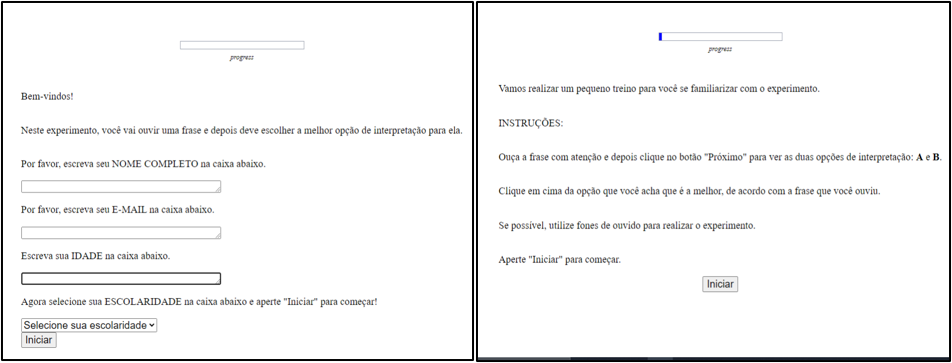
\includegraphics[width=0.9\textwidth]{fig-001.png}
 \caption{Primeira e segunda telas do experimento.}
 \label{fig1}
 \source{\emph{Print screen} da aplicação no navegador \emph{Google Chrome}.}
\end{figure}

\begin{figure}[htbp]
 \centering
 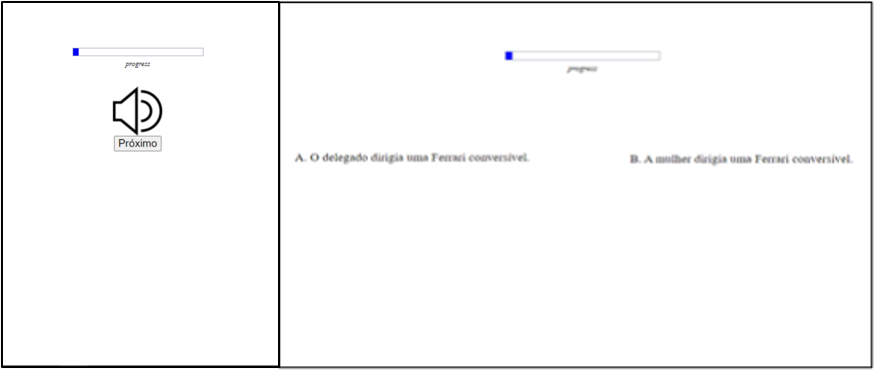
\includegraphics[width=0.9\textwidth]{fig-002.png} 
 \caption{Terceira e quarta telas do experimento\protect\footnotemark.}
 \label{fig2}
 \source{\emph{Print screen} da aplicação no navegador \emph{Google Chrome}.}
\end{figure}

\footnotetext{Não disponibilizamos \emph{print screen} da quinta e sexta telas porque as suas estruturação idênticas à da terceira e quarta telas.}

Para que nosso experimento pudesse ser estruturado e aplicado, portanto, a plataforma deveria ser capaz de: (i) suportar e executar áudios; (ii) recuperar as respostas dadas pelos respondentes; (iii) ser capaz de exibir textos e selecioná-los (através do teclado ou mouse); (iv) possibilitar a execução da estrutura do Quadrado Latino; e, (v) aplicar o experimento de forma \textit{online}. Esta última exigência surgiu posteriormente, ocasionada pelo distanciamento social imposto para o controle sanitário da pandemia de COVID-19.

Consideramos importante dedicar esta subseção para explicar as etapas do experimento executado porque temos ciência de que cada pesquisa tem características específicas, implicando, por isso, diferentes necessidades no que diz respeito aos programas dedicados à experimentação \textit{online}. Assim, deixamos claro que as avaliações a respeito dos programas apresentados na próxima subseção, bem como em nossa descrição da plataforma \emph{PCIbex}, são pautadas nas necessidades apresentadas durante o desenvolvimento da nossa pesquisa.

\subsection{\emph{PsychoPy} e \emph{PCIbex}}
Com o crescente uso da web para a realização de pesquisas científicas, diversos programas surgiram, visando não só tornar possível a experimentação em ambientes \textit{online}, mas, também, tornar o processo fácil para aqueles pesquisadores que não têm conhecimento na área de programação de computadores. Tendo em vista a quantidade de opções atualmente disponíveis, fazemos breve comparação com outro dos vários programas disponíveis, não só para ajudar futuros pesquisadores, mas, também, para contemplar, de maneira mais ampla, a plataforma \emph{PCIbex}. A escolha da plataforma experimental para essa comparação ocorreu pela sua aplicabilidade na área da Linguística experimental e pela característica comum de possibilidade de mensuração dos tempos de reação dos participantes em tarefas linguísticas comportamentais.

\subsubsection{\emph{PsychoPy}}
O \emph{PsychoPy} é um software gratuito e de código aberto que utiliza a linguagem de programação \emph{Python}. Foi desenvolvido em 2002, para atender, especificamente, necessidades de pesquisadores das áreas de Psicologia, da Psicofísica e da Neurociência, além de áreas interdisciplinares, como, por exemplo, a Psicolinguística. Esse programa tem como criador e principal contribuidor o pesquisador Jon Peirce \cite{peirce2007}.

Em comparação com o \emph{PCIbex}, essa plataforma pode ser usada tanto localmente quanto de forma \textit{online}. Isso amplia as possibilidades de uso dessa ferramenta, como, por exemplo, a sua utilização em conjunto de equipamentos de coleta de respostas fisiológicas, como o eletroencefalograma. Apesar disso, para ambos os usos (local ou \textit{online}), é necessário fazer a instalação do \emph{software}, que está disponível para Windows, Mac e Linux\footnote{Para instalar o PsychoPy é necessário acessar o site: \url{https://www.psychopy.org/}}.

Outra característica que o torna mais flexível em relação a outros programas são os seus dois módulos: o \emph{Coder}, voltado para programadores mais experientes com amplo conhecimento de \emph{Python}; e o \emph{Builder}, descrito por \textcite[p. 665]{limberger2019} como:  “Funcional e intuitivo, o referido módulo propicia a rápida aprendizagem do \emph{PsychoPy}”. O \emph{Builder} apresenta códigos mais simplificados, o que o torna ideal para pesquisadores sem muita experiência com programação.

Uma das vantagens do \emph{PsychoPy} sobre o \emph{Penn Controller} é o fato de separar os estímulos do \emph{script} principal do experimento. Além disso, o software gera os resultados do experimento em três extensões diferentes: “(1) log files - apresenta o \emph{output} cronológico de vários dados; (2) psydat - arquivo para análise em Python; e (3) arquivo com extensão .csv (comma separated value), para análise no programa estatístico R e/ou conversão no Excel” \cite[p. 667]{limberger2019}. O resultado de cada participante, porém, é gerado em arquivos individuais, o que acarreta o trabalho extra de unir todos os dados em uma única planilha, para análises globais.

Cumpre ressaltar que uma das grandes vantagens do \emph{PsychoPy} é o fato de haver ampla documentação a seu respeito, com fóruns, \emph{templates} e tutoriais, o que, certamente, contribui para a sua utilização por pesquisadores inexperientes em programação. Não obstante, \textcite[p. 682]{limberger2019} mencionam, em seu artigo, a existência de um tutorial em Português, produzido pela professora Mahayana Godoy, da Universidade Federal do Rio Grande do Norte \cite{tutorial}.

\subsubsection{PCIbex}
A \emph{PennController} for Ibex ou \emph{PCIbex}, assim como o outro programa mencionado, é uma plataforma gratuita e de código livre, desenvolvida por \textcite{zehr2018}. Seu funcionamento se baseia em outra ferramenta de elaboração de experimentos \textit{online}, no caso o \emph{Ibex Farm}, em relação ao qual funciona como uma biblioteca (\emph{library}), reunindo diversas funções prontas para uso. A extensão foi desenvolvida, especificamente, para a área de Psicolinguística, de forma semelhante ao \emph{PsychoPy}, que foi desenvolvido, especificamente, para a área de Psicologia.

É uma plataforma que funciona inteiramente \textit{online} e trabalha com uma mini linguagem própria, baseada, amplamente, na linguagem computacional \emph{JavaScript}\footnote{Pelo fato de a sua mini linguagem ser baseada em \emph{JavaScript}, ambas compartilham diversas semelhanças, como comandos e funções parecidas, como os comandos \emph{print}, \emph{var} e \emph{set}. Ressaltamos, entretanto, aqui, que, ainda assim, são duas linguagens diferentes; cada uma com suas particularidades.}. Nesse sentido, uma de suas vantagens é o fato de ter o próprio servidor, denominado \emph{PCIbex Farm}, no qual os experimentos são executados. Além disso, não necessita baixar qualquer tipo de programa, o que lhe assegura compatibilidade com qualquer computador e até mesmo celulares.

Apesar de não ter uma biblioteca extensa, como o outro programa citado, a \emph{PCIbex} tem um tutorial completo sobre como elaborar um experimento, criado pelos desenvolvedores dessa plataforma. Sua documentação apresenta um manual com explicações sucintas, mas suficientemente claras, sobre alguns dos seus componentes.

Uma desvantagem da \emph{PCIbex} é o fato de não trabalhar com estruturas condicionais; isto é: essa plataforma permite que seja exibido algum \emph{feedback} a partir da resposta do usuário para uma questão, mas não permite rodar um bloco de comandos a depender de uma resposta específica do participante, limitando uma série de usos que são possíveis no outro programa. Outro fator é quanto ao controle da participação de usuários, que permite que um respondente realize o experimento mais de uma vez, podendo esse procedimento ser prejudicial para os resultados de alguns tipos de tarefas experimentais ou acarretar em perda de participantes, devido à necessidade de descarte de participações em duplicidade.

Ainda assim, trata-se de uma plataforma muito recente, que vem passando por aprimorações. Por si mesma, a \emph{PCIbex} já é um exemplo de evolução, porque, comparativamente ao \emph{Ibex}, seu precursor, é muito mais fácil de manusear.

\section{\emph{Penn Controller} e experimentos}\label{sec-penncontroller}
A \emph{PCIbex}, como explicitado anteriormente, é uma plataforma totalmente gratuita e \textit{online}, de código aberto, desenvolvida para a realização de experimentos \textit{online}. Ela foi concebida pelos pesquisadores \textcite{zehr2018}, da University of Pennsylvania. É uma extensão, em forma de biblioteca, do programa \emph{Ibex}, desenvolvido por \textcite{drummond}. Foi lançada recentemente, em 2018, e, por isso, ainda não se encontra uma documentação extensa sobre ela; sobretudo em Português.

Para quem domina a língua inglesa, a \emph{Penn Controller} tem uma boa base de assistência ao usuário, que consiste em oferta de suporte, de um fórum de dúvidas e de tutoriais elaborados pelos desenvolvedores. Em língua portuguesa, como dissemos, o suporte ainda é incipiente. Por isso, acreditamos ser necessário explicitar, mais detalhadamente, o funcionamento dessa ferramenta, a fim de auxiliar aqueles pesquisadores que encontram dificuldades. Assim, dividimos o programa em duas partes: (1) a interface do \emph{PCIbex Farm}, na qual o usuário tem acesso aos documentos necessários para o funcionamento; e (2) os comandos básicos para a construção do \emph{script}, que é a estrutura principal do experimento\footnote{Aconselhamos consultar a documentação e o tutorial, em caso de qualquer dúvida, durante o desenvolvimento do seu experimento. Para questões mais específicas, sugerimos enviar um e-mail para o suporte ou escrever sobre a questão no fórum, que está indicado na parte inferior da página inicial do \emph{PCIbex Farm}.}.

\subsection{\emph{PCIbex Farm}}
O \emph{PCIbex Farm} é o servidor para os experimentos criados na \emph{PCIbex}. De acordo com a própria plataforma, atualmente existem mais de 2000 experimentos criados e hospedados nos servidores.

Em sua página inicial, o \emph{PCIbex Farm} oferece a possibilidade, com a opção “Empty project”, de se criar um novo experimento a partir do zero, ou, pelas opções “Masked Priming”, “Stroop Task”, “Self-Paced Reading”, “Covered Box Experiment”, “Mouse Tracking”, “MediaRecorder” e “EyeTracker”, de utilizar um dos modelos prontos, elaborados pelos desenvolvedores (\Cref{fig3}).

\begin{figure}[htbp]
 \centering
 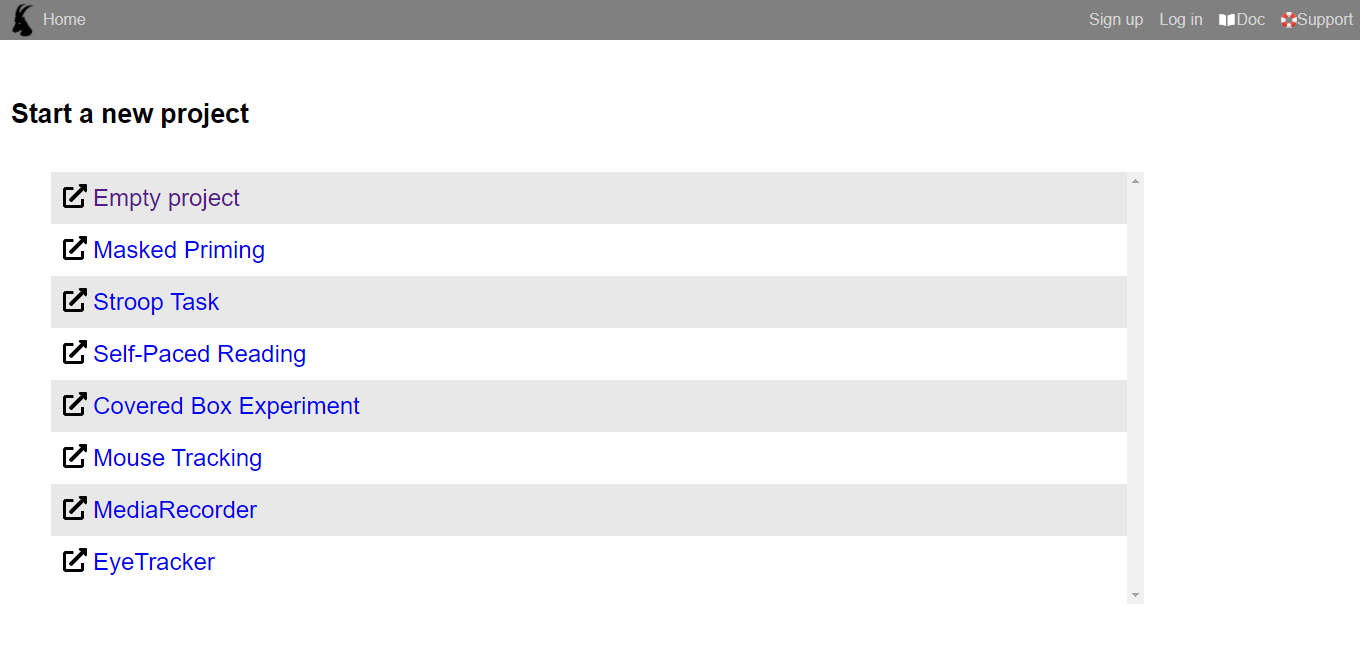
\includegraphics[width=0.9\textwidth]{fig-003.png}
 \caption{\emph{PCIbex Farm}.}
 \label{fig3}
 \source{\emph{Print screen} da aplicação no navegador \emph{Google Chrome}.}
\end{figure}

Além disso, tem-se, na parte superior da página, a opção de acessar, respectivamente, a página de \emph{sign up}; a página de \emph{login}; a documentação sobre a \emph{Penn Controller}; e, por fim, a área de suporte (\Cref{fig4}).

\begin{figure}[htbp]
 \centering
 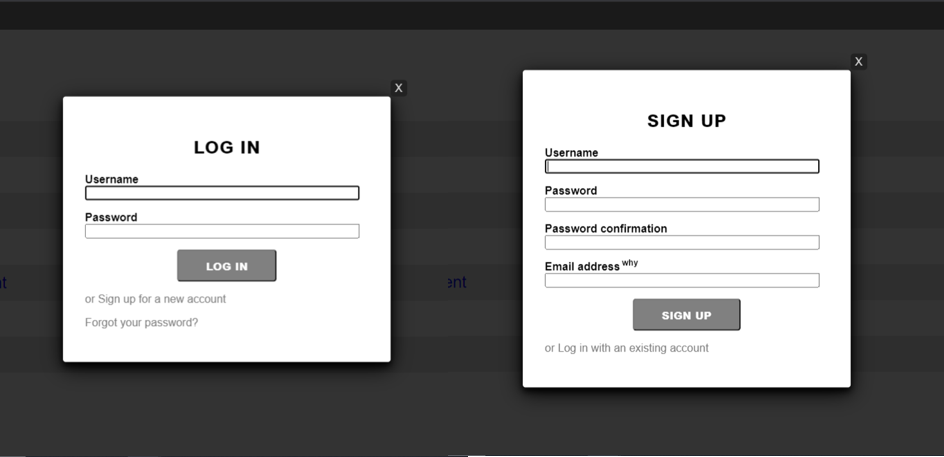
\includegraphics[width=0.9\textwidth]{fig-004.png}
 \caption{Telas de \emph{login} e \emph{sign up}.}
 \label{fig4}
 \source{\emph{Print screen} da aplicação no navegador \emph{Google Chrome}.}
\end{figure}

Após entrar no servidor, o usuário é direcionado para a página “projects”, na qual poderá criar e visualizar experimentos referentes a aquele \emph{login} (\Cref{fig5}).

\begin{figure}[htbp]
 \centering
 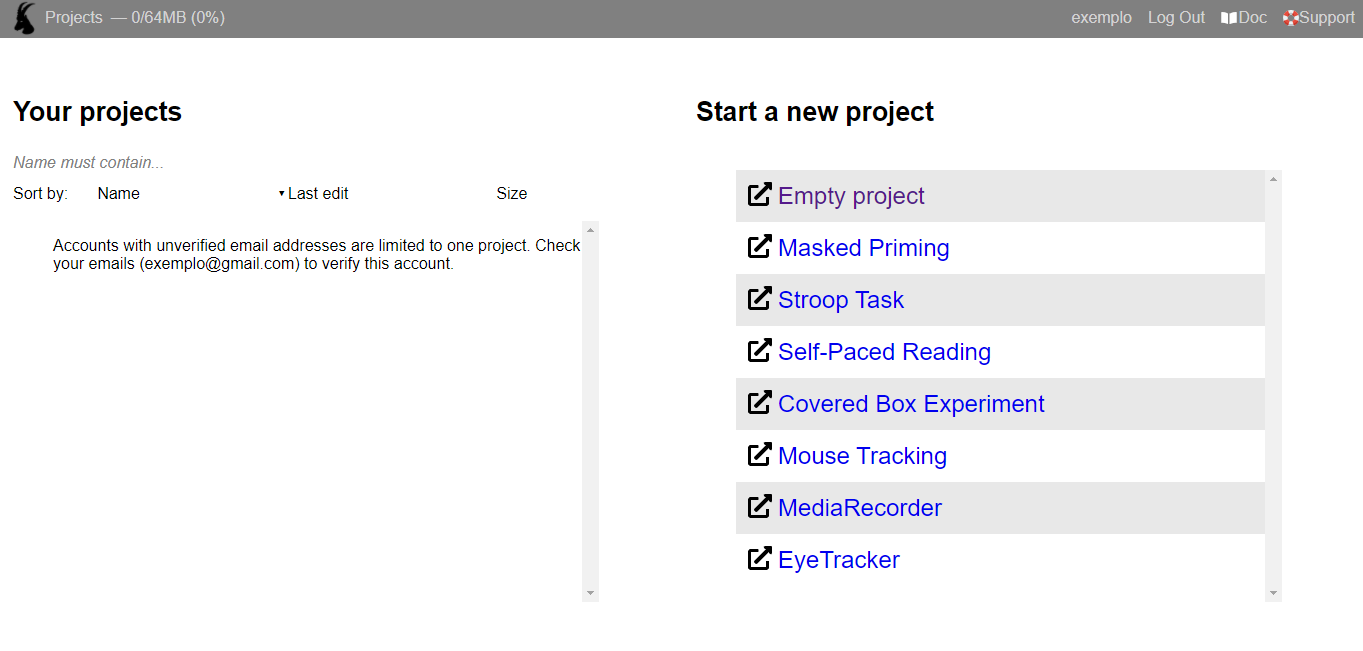
\includegraphics[width=0.9\textwidth]{fig-005.png}
 \caption{Tela "Projects".}
 \label{fig5}
 \source{\emph{Print screen} da aplicação no navegador \emph{Google Chrome}.}
\end{figure}

Para criar um experimento a partir do zero, o usuário deve clicar em “Empty project”. É possível, também, escolher iniciar um projeto dentre os modelos pré-concebidos ofertados pela plataforma. Os modelos são: “Masked Priming”, experimento no qual uma linha de caracteres aparece brevemente, antes de ser substituída por um texto, o qual o participante deve julgar se é uma palavra ou não; “Stroop Task”, tarefa na qual são apresentados termos sobre cores, como “vermelho”, “amarelo” e “azul”, escritos em cores não-correspondentes aos seus significados; “Self-Paced Reading”, teste de leitura auto monitorada, composto por duas sentenças; “Covered Box Experiment”, experimento no qual um áudio é apresentado ao participante, que deve informar se ele corresponde à imagem visível ou à imagem encoberta por um bloco; “Mouse Tracking”, teste no qual há o rastreamento do cursor (mouse)  do participante; Media Recorder”, tarefa na qual o participante deve pronunciar, em voz alta, o maior número possível de palavras, dentro do limite de tempo estipulado, que iniciem com a letra indicada; e, por fim, “Eye Tracker”, experimento no qual é realizado o rastreamento ocular do participante (\Cref{fig6}).

\begin{figure}[htbp]
 \centering
 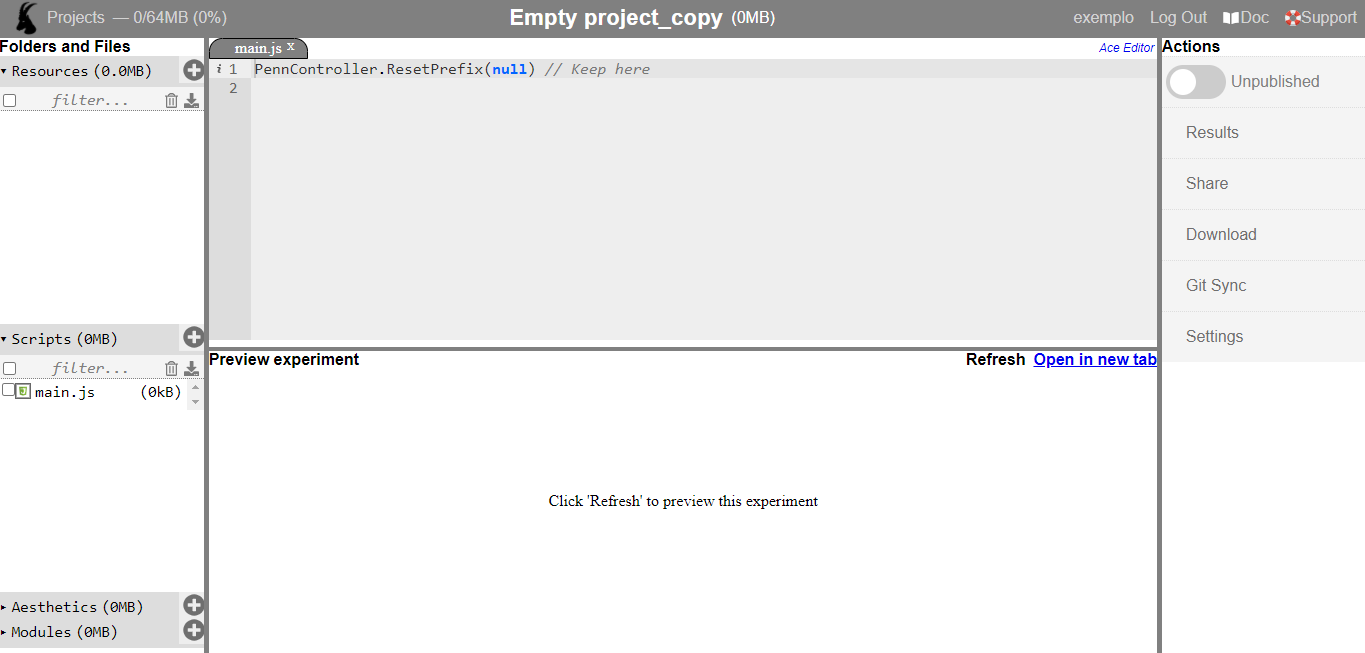
\includegraphics[width=0.9\textwidth]{fig-006.png}
 \caption{Tela “Projects” com um experimento criado.}
 \label{fig6}
 \source{\emph{Print screen} da aplicação no navegador \emph{Google Chrome}.}
\end{figure}

Depois de criado, o experimento é aberto, imediatamente, na página “Projects”, para que se possa iniciar a sua edição. A área de desenvolvimento do projeto é dividida em quatro seções, sendo elas: “Folders and Files”, “Ace Editor”, “Preview experiment” e “Actions”.

Na seção “Folders and Files”, temos quatro abas: “Resources”, “Scripts”, “Aesthetics” e “Modules”. Para não estendermos a nossa explicação, porém, focamos apenas as duas primeiras, que se configuram essenciais para a elaboração do experimento.

A primeira aba, “Resources”, é uma das mais utilizadas pelo pesquisador, porque é nela que são colocados todos os estímulos e tabelas, mas é a segunda aba, “Scripts”, a mais importante, sendo a seção na qual o \emph{script} principal fica armazenado; isto é: a estrutura base do experimento se encontra nela.  

Em “Ace Editor” e “Preview experiment”, o pesquisador pode, respectivamente, editar ou visualizar os documentos selecionados em “Folders and Files” e pode conferir uma prévia do experimento, sem precisar abri-lo em uma nova página no navegador.

Já em “Actions”, além de poder conferir o arquivo de resultados gerado na aba “Results” (em formato .csv), é possível, também, encontrar o link de acesso que deve ser enviado aos participantes da pesquisa, localizado em “Share”.

Ao clicar em “Share”, o usuário irá se deparar com dois links, um somente para testes, no qual é possível averiguar a condição da estrutura criada, denominado “Demonstration link” e, outro, para a efetiva coleta de dados, nomeado de “Data-collection link”. Cumpre notar que esse segundo só funciona quando o experimento for publicado; isto é: quando seu status for alterado para “Published”. Para publicar um experimento, o pesquisador deve clicar no primeiro botão que aparece em “Actions”.

Na seção em questão, pode-se, também, acessar a aba “Git Sync”, que é responsável por conferir o acesso a repositórios externos do Github. Essa ferramenta se mostra extremamente necessária para pesquisas com estímulos de vídeos e/ou áudios, já que a \emph{PCIbex} suporta apenas 64MB de dados (\Cref{fig7}).

\begin{figure}[htbp]
 \centering
 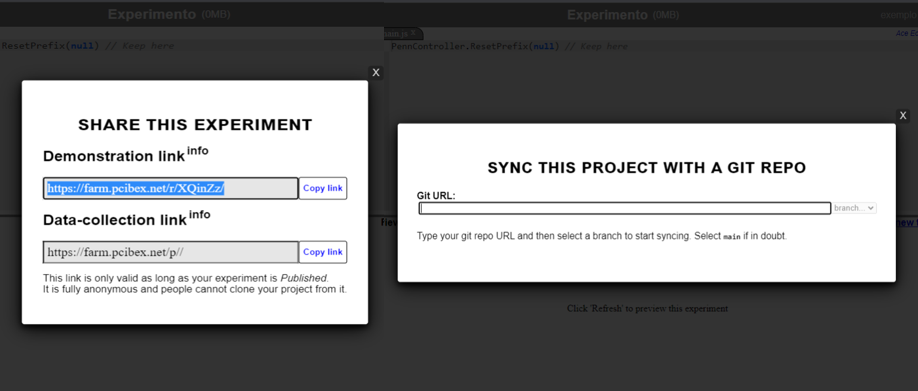
\includegraphics[width=0.9\textwidth]{fig-007.png}
 \caption{Aba “Share” e “Git Sync”.}
 \label{fig7}
 \source{\emph{Print screen} da aplicação no navegador \emph{Google Chrome}.}
\end{figure}

Depois de criado, de volta à tela inicial da página “Projects”, o experimento apresentará as opções de testar o experimento "Try it", de criar uma cópia do experimento "Clone", de nomeá-lo novamente "Rename" e de excluí-lo "Delete". Para acessá-lo novamente, basta clicar em seu nome (\Cref{fig8}).

\begin{figure}[htbp]
 \centering
 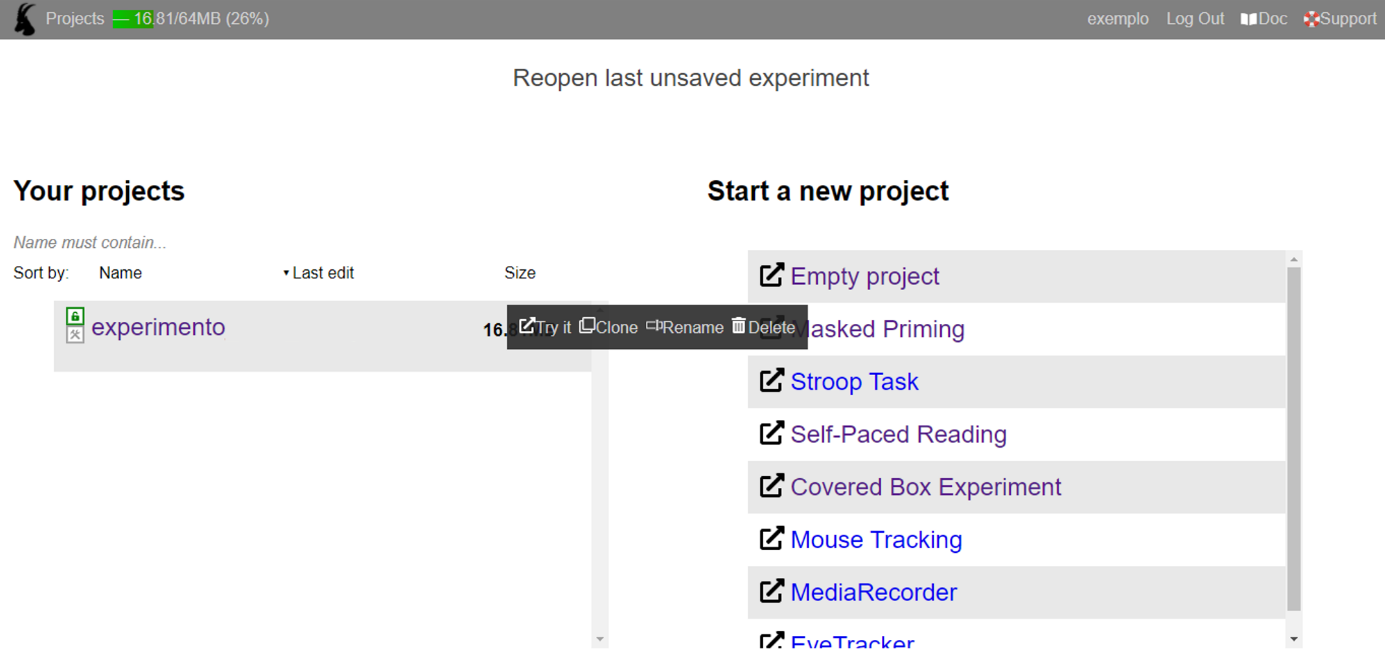
\includegraphics[width=0.9\textwidth]{fig-008.png}
 \caption{Tela inicial do experimento.}
 \label{fig8}
 \source{\emph{Print screen} da aplicação no navegador \emph{Google Chrome}.}
\end{figure}

\subsection{Comandos}
A \emph{PCIbex} tem diversos comandos, visando atender o maior número possível de experimentos na área de Psicolinguística. Tem, também, uma excelente, apesar de pequena, documentação sobre os comandos e suas possibilidades. Tratamos, neste artigo, dos comandos fundamentais para a elaboração de um experimento.

\subsubsection{\emph{New Trial} e \emph{Sequence}}
O comando “newTrial” é utilizado para criar uma nova tela, enquanto o comando “Sequence” é utilizado para organizar em que ordem essas páginas irão aparecer. Os dois juntos definem a estrutura base do experimento. Enquanto o primeiro irá conter outros comandos que realizam ações como exibir textos, exibir botões, salvar informações, etc., o segundo terá como \emph{input} somente os nomes atribuídos a cada “newTrial” (com exceção de alguns comandos específicos para randomizar itens ou salvar resultados previamente). Além disso, \textcite{zehr2018} recomendam que, antes de se começar a programar o \emph{script}, o pesquisador planeje a quantidade de telas que o experimento necessitará, para que já tenha em mente quantos “newTrial” serão necessários. Abaixo apresentamos um exemplo do uso do comando “Sequence”, no qual é definida a ordem de seis telas, além de randomizar os itens da tela “experiment” e gravar os resultados coletados antes da exibição da tela “final” (com a utilização do comando “SendResults”) (\Cref{fig9}).

\begin{figure}[htbp]
 \centering
 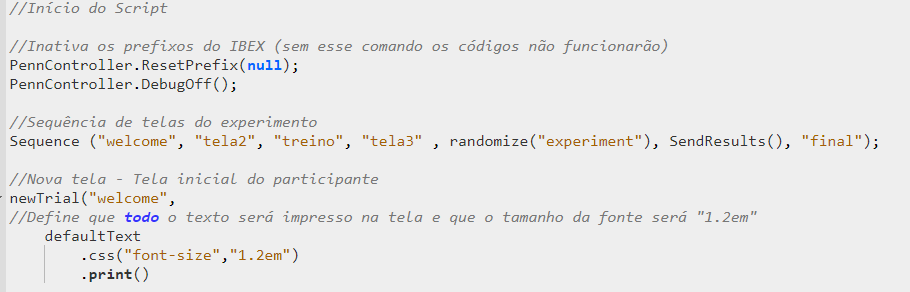
\includegraphics[width=0.9\textwidth]{fig-009.png}
 \caption{Comando “Sequence”.}
 \label{fig9}
 \source{\emph{Print screen} da aplicação no navegador \emph{Google Chrome}.}
\end{figure}

A \Cref{fig10} exemplifica a utilização de um “newTrial”, o qual criará uma nova tela, intitulada “tela2”, que exibirá uma série de textos contendo as instruções para a fase de treino do experimento, além de um botão que possibilita ao participante avançar para a próxima tela.

\begin{figure}[htbp]
 \centering
 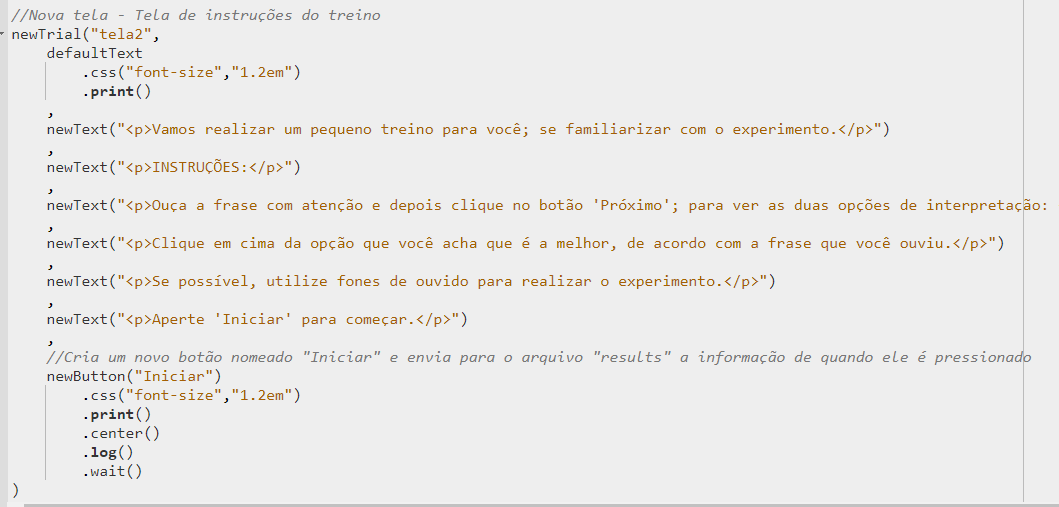
\includegraphics[width=0.9\textwidth]{fig-010.png}
 \caption{Comando “newTrial”.}
 \label{fig10}
 \source{\emph{Print screen} da aplicação no navegador \emph{Google Chrome}.}
\end{figure}

\subsubsection{\emph{Template}}
A \emph{PCIbex} tem uma característica particular que é: utilizar tabelas para definir a relação entre os estímulos e as opções de resposta. Por isso, um dos seus comandos mais importantes é o “Template” que executa cada linha de uma tabela, de extensão .csv, como um “trial”, tornando possível a execução de todos os estímulos e as suas opções de resposta correspondentes.

Para exemplificar como montar uma tabela corretamente, apresentamos a estrutura da tabela feita para a tarefa experimental de nossa pesquisa sobre focalização e adjuntos adverbiais. Para o nosso experimento, necessitávamos que a tabela possuísse todos os nossos 80 áudios de estímulo, 84 áudios com as sentenças distratoras (já que são 21 distratoras para cada grupo) e todas as opções de resposta, além da opção que esperávamos que o participante respondesse. Dessa forma, a tabela que construímos tinha 6 colunas e 165 linhas (devido ao cabeçalho da tabela). Essas seis colunas eram respectivamente: “Audiofile”, na qual estavam listados os áudios de estímulo; “OptionA”, na qual estavam listadas as opções “A” de interpretação; “OptionB”, na qual estavam listadas as opções “B” de interpretação; “Item”, os estímulos estavam identificados por um código que elaboramos; "Group", que determinada a distribuição dos itens em 4 grupos de participantes, seguindo a distribuição por Quadrado Latino; e “RespostaEsperada”, na qual tinha-se a informação de quais das duas opções esperávamos que o respondente escolhesse de acordo com as condições experimentais do item (\Cref{fig11}).

\begin{figure}[htbp]
 \centering
 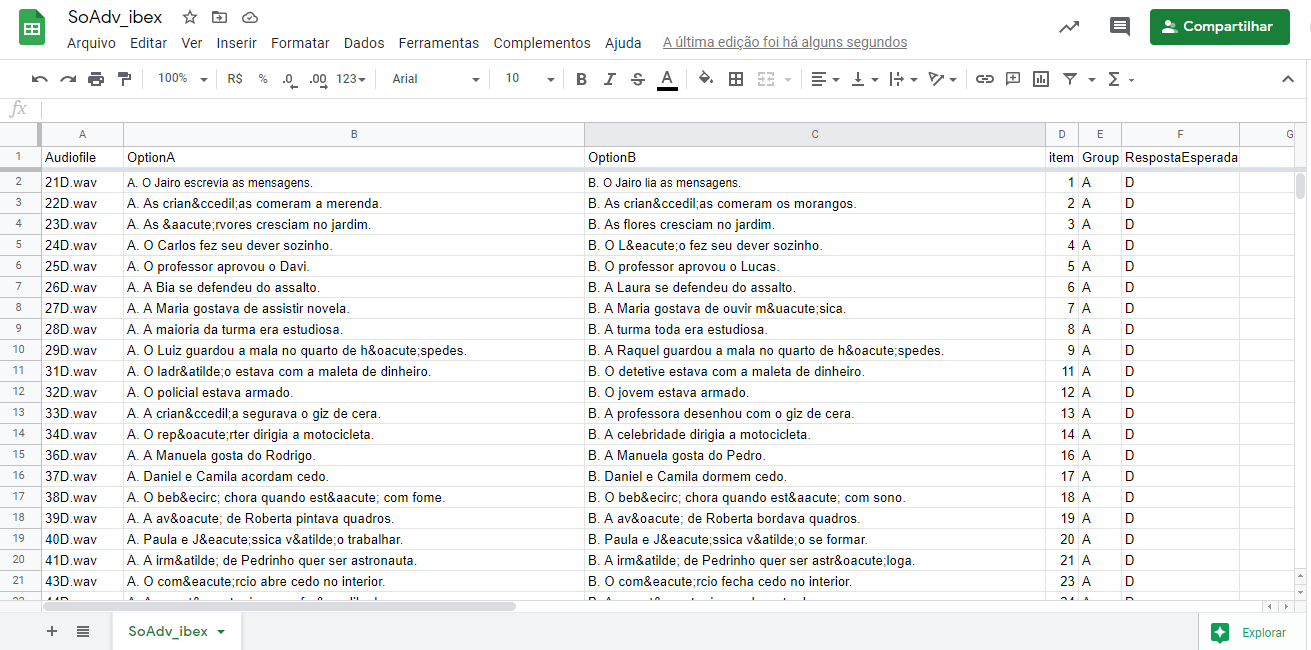
\includegraphics[width=0.9\textwidth]{fig-011.png}
 \caption{Tabela utilizada no nosso experimento.}
 \label{fig11}
 \source{\emph{Print screen} da aplicação “google planilhas” no navegador Google Chrome.}
\end{figure}

A coluna “Group” é um caso à parte, porque ela é a única coluna estritamente obrigatória, caso a pesquisa use mais de uma versão do estímulos ou utilize o Quadrado Latino. Nessa coluna é colocado o número ou a letra da versão ao ou à qual correspondem os estímulos e as respostas. A \emph{PCIbex} reconhece, automaticamente, a coluna e escolhe, de forma aleatória, qual versão exibir para o participante. É válido ressaltar que não se pode alterar o título da coluna, senão a \emph{PCIbex} não a reconhecerá.

Ainda sobre o comando “Template”, ele deve conter o nome completo da tabela – isto é: o nome da tabela e a sua extensão (exemplo: “SoAdv\_ibex.csv”) – e um “newTrial” onde se escreverá de fato o código para executar os estímulos e exibir as respostas. O “trial” deve ser precedido pelo comando “variable” ou “row”. Esses comandos só aparecem em conjunto com o comando “Template” e são eles que possibilitam que todas as linhas da tabela sejam lidas (\Cref{fig12}).

\begin{figure}[htbp]
 \centering
 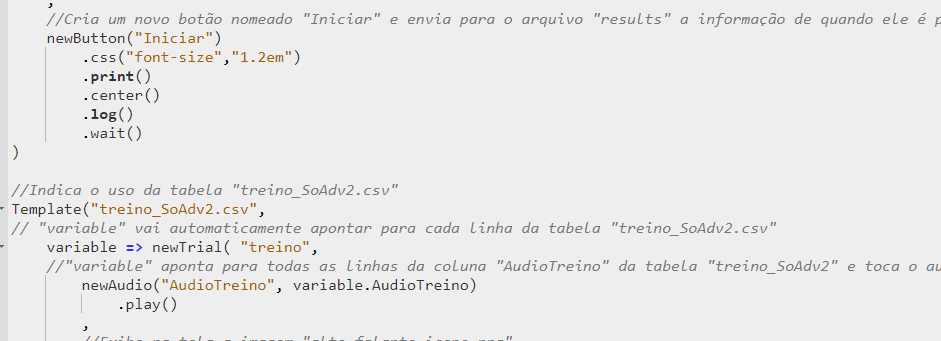
\includegraphics[width=0.9\textwidth]{fig-012.png}
 \caption{Comando “Template”.}
 \label{fig12}
 \source{\emph{Print screen} da aplicação no navegador \emph{Google Chrome}.}
\end{figure}

\subsubsection{Elementos}
Elementos são comandos que inserem componentes visuais ou de áudio no \emph{script}. Existem dois tipos desses elementos: aqueles que pedem uma interação com o participante e aqueles que não a pedem.

Do primeiro tipo, podemos citar os elementos: “Button”, que cria um botão, com possibilidades variadas de funções; “DropDown”, que exibe uma caixa de seleção na qual as opções são exibidas em forma de lista vertical; “TextInput”, que cria uma caixa de texto; “Key”, que possibilita a utilização do teclado, ao invés da criação de um botão; e “Selector”, que permite que o participante selecione imagens, textos, etc., usando-se o cursor do mouse (\Cref{fig13}).

\begin{figure}[htbp]
 \centering
 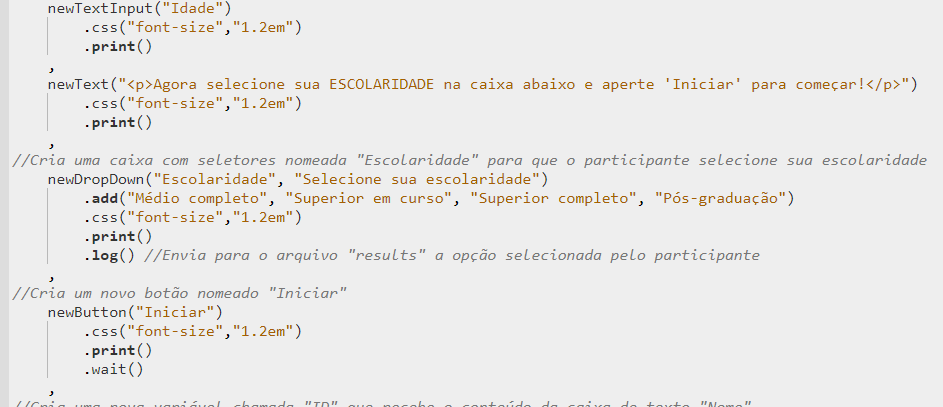
\includegraphics[width=0.9\textwidth]{fig-013.png}
 \caption{Comandos “newDropDown”, “newTextInput” e “newButton”.}
 \label{fig13}
 \source{\emph{Print screen} da aplicação no navegador \emph{Google Chrome}.}
\end{figure}

Já no segundo tipo, temos os elementos “Text”, “Audio”, “Image” e “Video”, que exibem ou reproduzem, respectivamente, textos, áudios, imagens e vídeos. O elemento “Canvas” funciona de maneira diferente, já que não exibe as mídias, especificamente, mas as dispõe em uma localização espacial na tela de exibição do experimento definida pelo pesquisador. Esse elemento é essencial para a utilização de imagens, para que elas possam ser colocadas lado a lado, por exemplo (\Cref{fig14}).

\begin{figure}[htbp]
 \centering
 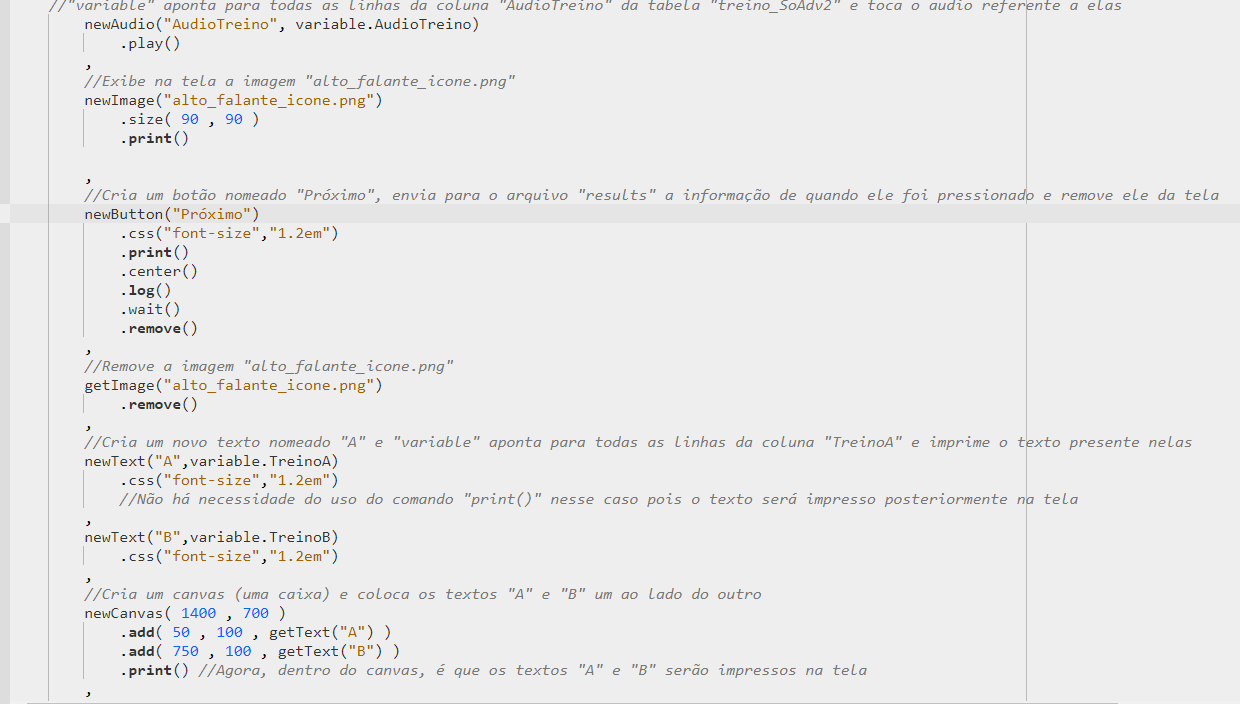
\includegraphics[width=0.9\textwidth]{fig-014.png}
 \caption{Comandos “newAudio”, “newImage”, “newText” e “newCanvas”.}
 \label{fig14}
 \source{\emph{Print screen} da aplicação no navegador \emph{Google Chrome}.}
\end{figure}

Ainda existem outros elementos que não citamos aqui, por serem de usos mais específicos. Ressaltamos, portanto, a importância de se consultar a documentação oficial e o tutorial disponíveis no site da \emph{PCIbex}, quando o pesquisador se deparar com necessidades específicas para a programação do seu experimento em particular.

\subsubsection{Print}
O comando “print”, diferentemente dos comandos apresentados acima, é frequentemente utilizado dentro de outros elementos, que podem ser elementos de texto, de botão, de imagem, de caixa de seleção, etc.. Sua função é exibir qualquer elemento no qual ele tenha sido declarado. Assim, um texto só aparecerá na tela se a ele estiver atribuído o comando “print”. Na imagem abaixo (\Cref{fig15}), apresentamos um exemplo do uso do comando para “imprimir” um texto, uma caixa de seleção e um botão na tela.

\begin{figure}[htbp]
 \centering
 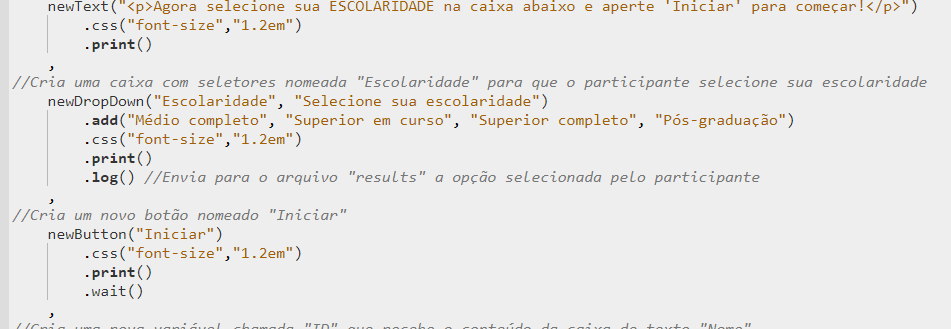
\includegraphics[width=0.9\textwidth]{fig-015.png}
 \caption{Comando “print”.}
 \label{fig15}
 \source{\emph{Print screen} da aplicação no navegador \emph{Google Chrome}.}
\end{figure}

\subsubsection{Wait}
Normalmente, a \emph{PCIbex} percorrerá todo o \emph{script}, linearmente, caso ele não apresente erros de digitação ou sintaxe. Dessa forma, se um elemento é exibido na tela por um comando “print”, ele desaparecerá, imediatamente depois, quando a ferramenta ler a linha de comando seguinte. Como esse processamento é feito em questão de milissegundos, em alguns casos específicos será necessário manter o elemento na tela por mais tempo, até que o participante execute uma ação, por exemplo. Para isso, o comando “wait”, permite que a aplicação só processe a linha seguinte após alguma interação do participante com o elemento no qual ele está contido (normalmente, um elemento do tipo botão ou do tipo seletor). Assim, todos os elementos exibidos anteriormente no escopo do comando “wait” permanecerão na tela, aguardando a ação do participante ou um novo comando que anule a ação de espera (\Cref{fig16}).

\begin{figure}[htbp]
 \centering
 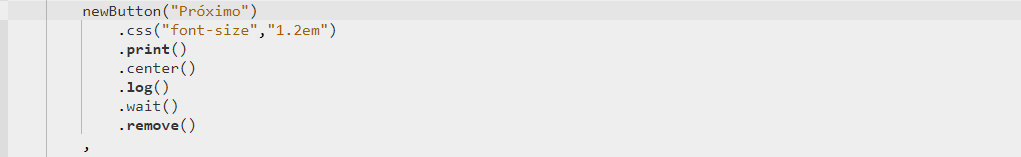
\includegraphics[width=0.9\textwidth]{fig-016.png}
 \caption{Comando “wait”.}
 \label{fig16}
 \source{\emph{Print screen} da aplicação no navegador \emph{Google Chrome}.}
\end{figure}

\subsubsection{Log}
De forma semelhante ao “print” e ao “wait”, o comando “log” não terá outros comandos como conteúdo e será declarado em elementos para os quais se faz necessário gravar alguma informação fornecida pelo participante. Assim, a função do “log” é salvar informações, que depois constarão no arquivo de resultados (\Cref{fig17}).

\begin{figure}[htbp]
 \centering
 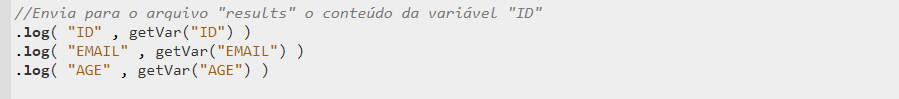
\includegraphics[width=0.9\textwidth]{fig-017.png}
 \caption{Comando “log”.}
 \label{fig17}
 \source{\emph{Print screen} da aplicação no navegador \emph{Google Chrome}.}
\end{figure}

\subsection{Nossa experiência utilizando a \emph{PCIbex}}
Tratamos, neste artigo, até aqui, de visões gerais sobre a plataforma \emph{PCIbex} e de detalhes sobre a sua funcionalidade. Explicitamos, agora, a nossa experiência com o uso da plataforma, quais foram as dificuldades e as facilidades, o que aprendemos durante o processo, bem como as vantagens e desvantagens que encontramos ao utilizar essa plataforma.

Antes de prosseguir, ressaltamos que, apesar de os comandos utilizados pela plataforma não se mostrarem extremamente complicados, ter alguma experiência em programação facilita muito o processo. No nosso caso, uma das autoras tem formação técnica em Informática e, apesar de as outras duas serem leigas, no sentido de não terem formação específica na área, uma delas tem ampla experiência com programação com outras ferramentas, como o DMDX \cite{forster2002}, o que possibilitou obter diversas visões sobre o desenvolvimento do experimento no \emph{Penn Controller}.

Nesse sentido, para pesquisadores sem experiência com programação, o tutorial e a documentação oferecidos pelo site, embora concisos, são extremamente elucidativos. Durante a construção do experimento, a consulta a ambos os conteúdos foi essencial, facilitando muito o nosso trabalho. Esperamos, também, que as descrições trazidas neste artigo sirvam como facilitadoras para o início do processo de programação para pesquisadores menos experientes.

Uma das dificuldades que enfrentamos foi com relação aos carregamentos dos áudios, que, por diversas vezes, travaram ou demoraram demasiadamente a serem executados. Devido a isso, alguns participantes reportaram tribulações para realizar, até o final, a tarefa do experimento.

Além disso, a plataforma tem certas particularidades que não podem ser consideradas empecilhos, mas eram, definitivamente, incômodas durante o processo de criação do \emph{script}. Um exemplo disso é o tamanho reduzido da base de dados para o experimento. Mesmo a plataforma oferecendo uma solução para essa questão – nesse caso, a sincronização com um repositório externo do GitHub –, essa sincronização apresentava falhas, acabando por efetivamente ocupar o espaço na base de dados. Para que a solução de usar um repositório externo pudesse, de fato, funcionar em alguns casos de itens experimentais muito extensos, foi necessário adicionar ao \emph{script} um comando extra de acesso direto ao repositório, ao invés de utilizar a aba na seção “Actions”.

Em relação ao funcionamento da coluna “Group”, de início o mecanismo contribuiu muito para a agilidade do processo, mas ocorreu algum erro no servidor\footnote{Não sabemos exatamente qual foi o problema que resultou na distribuição desigual dos grupos. A probabilidade maior é a de que, devido às condições instáveis de Internet tenha ocorrido um erro no momento de o servidor registrar qual grupo já tinha sido distribuído.}, durante o controle do número de participantes para cada versão do experimento, resultando em um número desigual de respondentes em cada grupo. No final, acabamos separando os quatro grupos em quatro \emph{scripts} diferentes; depois, os enviamos a um número exato de pessoas, a fim de termos um número balanceado e controlado de participantes em cada grupo.

Apesar dessas dificuldades e aparentes desvantagens, sem a plataforma seria impossível aplicarmos o nosso experimento e dar continuidade à pesquisa no período de distanciamento social. Além disso, o fato de a plataforma ser totalmente gratuita e \textit{online} contribuiu muito para que pudéssemos utilizá-la sem problemas e à distância. A agilidade com que conseguimos montar o nosso experimento e aplicá-lo foi essencial, já que não tínhamos planejado utilizar essa ferramenta antes de a pandemia do novo Coronavírus ocorrer.

Dessarte, graças à linguagem simples com a qual a plataforma opera e à sua praticidade, realizamos um experimento no prazo de um mês, sem ter tido qualquer contato prévio com a aplicação e, mesmo com os obstáculos apresentados, devido ao seu caráter flexível, conseguimos aplicar nosso experimento sem termos de fazer qualquer adaptação estrutural, implementando-o da forma como havíamos planejado.
	
Os resultados coletados a partir do nosso experimento foram extremamente positivos, relativo à qualidade e à análise desses. Devido à possibilidade de acessarmos rapidamente os resultados e conferir dados da coleta – como, por exemplo, possíveis erros de execução e levantamento do número de participantes por grupo experimental –, conseguimos garantir que houvesse um bom número de participantes em cada grupo, apesar de termos tido 8 (oito) participantes com problemas na execução dos áudios.

Ainda sobre os resultados, a conversão automática do arquivo em uma tabela separada por vírgulas (.csv) tornou mais rápido o processo de análise dos dados. Nesse formato, é possível exportar o arquivo para programas como o Excel, que possibilitam a aplicação de filtros para a organização dos dados antes da realização de análises estatísticas descritivas e inferenciais.

Por fim, cumpre-nos relatar que, durante a criação do nosso experimento, deparamo-nos com outros problemas e \emph{bugs}, não registrados neste artigo, porque foram recentemente identificados, analisados e corregidos pelos desenvolvedores da plataforma. Isso é o resultado do aprimoramento diligente e do comprometimento que \textcite{zehr2018} têm no sentido tornarem essa plataforma cada vez mais acessível e inclusiva para pesquisadores de diversas partes do mundo, com diferentes níveis de conhecimento.

Acreditamos que a \emph{PCIbex} tem muito futuro e pode se tornar uma ferramenta crucial para pesquisadores das áreas de Ciências Humanas, Sociais Aplicadas e de Linguística experimental, principalmente em tempos de isolamento social. A pesquisa \textit{online}, como um todo, é uma alternativa que deve começar a ser mais considerada pela comunidade acadêmica. Não é apenas uma “solução de última hora”, mas uma opção para redução de custos e de tempo na formulação de experimentos, além de ter potenciais de alcance e interação muito maiores com os participantes.

\section{Considerações finais}
A evolução da internet criou um novo universo que ainda não é tão aproveitado quanto é possível. Tomamos como base a nossa pesquisa, que não precisaria de uma plataforma que possibilitasse a aplicação de um experimento via web, se não fosse a pandemia do novo Coronavírus. A partir da necessidade emergencial, recorremos aos instrumentos disponíveis.

Mesmo partindo desse contexto, defendemos que a internet é elemento facilitador para pesquisas, não só por oferecer ferramentas básicas e essenciais, como o e-mail, mas também por possibilitar o desenvolvimento de outras, mais complexas, como as que são mencionadas neste artigo. Salientamos que os direcionamentos éticos que regem o desenvolvimento científico também se aplicam a qualquer tipo de pesquisa via web. Ainda com muito a ser explorado, esse cenário é promissor.

Nesse sentido, plataformas que oferecem a possibilidade de aplicar experimentos de forma \textit{online} tornam-se grandes aliadas do pesquisador, agilizando processos e diminuindo gastos. A documentação existente sobre essas ferramentas, porém, ainda é escassa, por vezes podendo excluir pesquisadores que não tenham conhecimentos na área de programação, ou aqueles que não tenham domínio suficiente da língua inglesa, língua na qual a maior parte dos tutoriais sobre essas aplicações está escrito.

Essas considerações se aplicam à ferramenta que utilizamos para realizar o nosso experimento, a \emph{Penn Controller} para o \emph{Ibex}. A \emph{PCIbex}, além de ter se adequado às nossas necessidades (precisávamos de um programa que possibilitasse a criação de um experimento qualitativo e quantitativo, com áudio, seleção de opções e registro de tempo de resposta), também apresentou diversas vantagens, quando comparada a outras aplicações, como o \emph{PsychoPy}.

A partir do que foi elencado acima, procuramos, neste artigo, elucidar as vantagens da utilização do ambiente web para a realização de pesquisas na área de Psicolinguística experimental, além de incentivar a construção de experimentos na plataforma \emph{PCIbex}, que foi uma grande facilitadora para a aplicação do nosso experimento.

Assim, esperamos contribuir, por meio desse trabalho, com outros pesquisadores brasileiros que buscam elaborar pesquisas \textit{online}, a fim de que possam utilizá-lo como um guia inicial para a escolha e o uso da plataforma \emph{PCIbex} em suas atividades experimentais.


\printbibliography\label{sec-bib}
% if the text is not in Portuguese, it might be necessary to use the code below instead to print the correct ABNT abbreviations [s.n.], [s.l.] 
%\begin{portuguese}
%\printbibliography[title={Bibliography}]
%\end{portuguese}

%full list: conceptualization,datacuration,formalanalysis,funding,investigation,methodology,projadm,resources,software,supervision,validation,visualization,writing,review
\begin{contributors}[sec-contributors]
\authorcontribution{Aline Alves Fonseca}[projadm,resources,supervision,review]
\authorcontribution{Júlia Greco Carvalho}[conceptualization,investigation,software,visualization,writing]
\authorcontribution{Samara Cristina da Silva Zanella}[conceptualization,investigation,visualization,writing]
\end{contributors}


\end{document}
